\chapter{Noțiuni teoretice}

\section{Rețele Neurale Recurente}

Rețelele neuronale recurente (RNN - Recurent Neural Networks) sunt o arhitectura aparte de rețele neuronale, ce le face atat de speciale este faptul ca ele reușesc sa capteze secvențialitatea datelor. Ele sunt folosite in special în procesarea limbajului natural, dar și în procesarea imaginilor, a seriilor de timp, a recomandarilor de produse. Cu alte cuvinte oricând vine vorba de succesiunea anumitor evenimente, ele reprezintă un candidat bun în captarea acestor modele in date.

Figura \ref{fig:rnn_arch} prezintă arhitectura unei rețele recurente, unde fiecare dreptunghi ține locul stratului ascuns de la pasul, $t$. Fiecare strat ascuns este format din perceptroni care execută operația de inmulțire intre parametrii și input, urmată de o operație nonlineară (ex.$ tanh$). La fiecare pas din timp, ieșirea de la pasul anterior, împreună cu vectorul următorului cuvânt, $x_t$, sunt intrări în stratul ascuns care produce pentru pasul următor, iețirea $y$, și vectorul de caracteristici al stratului ascuns, $h$.


\begin{equation}
	h_t = \sigma{(W^{(hh)} h_{t-1} + W^{(hx)} x_{[t]})}
	\label{h_t}
\end{equation}

\begin{equation}
	y_t = softmax(W^{(S)} h_t) 
	\label{y_t}
\end{equation}

\begin{figure}[h]
	\centering
	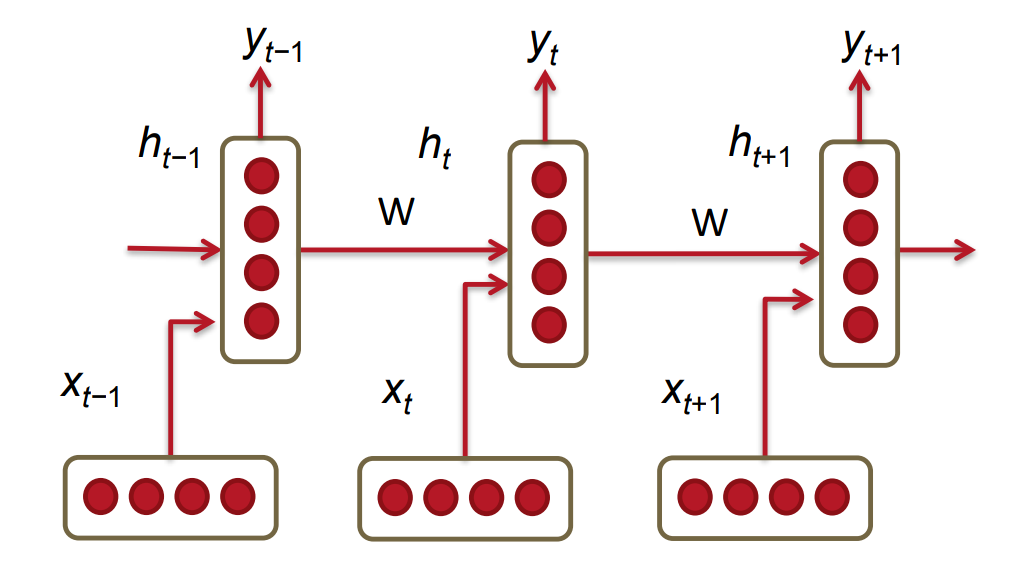
\includegraphics[scale=0.3]{rnn_arch.png}
	\caption{Arhitectura RNN \cite{cs224d_notes}}
	\label{fig:rnn_arch}
\end{figure}

Descrierea parametrilor din rețea:

\begin{itemize}
	\item $x_1, x_2, ..., x_T$ vectorii cuvintelor dintr-o secvență de lungime $T$
	\item $h_t = \sigma{(W^{(hh)} h_{t-1} + W^{(hx)} x_{[t]})}$: formula care descrie calculul vectorului de caracteristici, $h_t$, la fiecare pas $t$:
	
	\begin{itemize}
		\item $ x_t \in {\rm I\!R}^d $ vectorul cuvântului $t$
		\item $ W^{hx} \in {\rm I\!R}^{D_h \times d} $ matricea ponderilor utilizată la condiționarea vectorului de intrare, $x_t$
		\item $ W^{hh} \in {\rm I\!R}^{D_h \times D_h} $ matricea ponderilor utilizată la condiționarea ieșirii de la pasul anterior, $h_{t-1}$
		\item $ h_{t-1} \in  {\rm I\!R}^{D_h} $ ieșirea funcției nonlineare de la pasul anterior, $t-1$, iar $h_0 \in  {\rm I\!R}^{D_h}$ este vectorul de inițializare pentru stratul ascuns, la pasul $t=0$
		\item $ \sigma() $ funcția nonlineară  (sigmoid in acest exemplu)
	\end{itemize}

	\item $ y_t = softmax(W^{(S)} h_t) $ ieșirea care reprezintă o distribuție de probabilitate peste vocabular la fiecare pas $t$. În esență, $y_t$ este următorul cuvânt prezis, dându-se contextul de până  acum ($ h_{t-1} $) și ultimul cuvânt observat ($x_t$). Avem  $ W^{S} \in {\rm I\!R}^{|V| \times D_h} $ și $ y \in {\rm I\!R}^{|V|} $, unde $|V|$ reprezintă cardinalitatea mulțimii $V$ adică a vocabularului de cuvinte.

\end{itemize}

Funcția de cost utilizată in rețelele neuronale recurente este de obicei CE (cross entropy error).

Pentru pasul $t$:
$$
J_{(t)}(\theta) = - \sum_{j=1}^{|V|}  ytrue_{t, j} \times \log(y_{t, j})
$$

% todo sa investighez de ce nu dispare minusul, eroare in formula
Pentru toată secvența de lungime $T$ funcția de cost devine:
$$
J = - \frac{1}{T} \sum_{t=1}^{T} J_{(t)}(\theta) = - \frac{1}{T} \sum_{t=1}^{T}  \sum_{j=1}^{|V|}  ytrue_{t, j} \times \log(y_{t, j})
$$

\cite{cs224d_notes}


\subsection{Problema diminuării si a exagerării gradientului}
O RNN împarte aceeași matrice a parametrilor pentru toată secvența de intrare. Țelul unei astfel de arhitecturi este acela de a capta contextul și în cazul secvențelor de lungimi mai mari.

Considerăm ecuațiile \ref{h_t} și \ref{y_t} de mai sus la pasul $t$. Pentru a calcula eroarea unei RNN, $dE/dW$, vom însuma erorile de la fiecare pas de timp.

\begin{equation}
	\frac{\partial E}{\partial W} = \sum_{t=1}^{T} \frac{\partial E_t}{\partial W}
\end{equation}

Eroarea la fiecare pas de timp este calculată prin diferențierea ecuațiilor  \ref{h_t} și \ref{y_t}:

\begin{equation}
	\frac{\partial E_t}{\partial W} = \sum_{k=1}^{t} \frac{\partial E_t}{\partial y_t} \frac{\partial y_t}{\partial h_t} \frac{\partial h_t}{\partial h_k} \frac{\partial h_k}{\partial W}
	\label{chain_rule_E}
\end{equation}

Unde $\frac{dh_t}{dh_k}$ este derivata parțială a stării ascunse $h_t$ în raport cu toți $k$ pași de timp anteriori.

\begin{equation}
	\frac{\partial h_t}{\partial h_k} = \prod_{j=k+1}^{t} \frac{\partial h_j}{\partial h_{j-1}} = \prod_{j=k+1}^{t} W^T \times diag[f'(j_{j-1})]
	\label{chain_rule_prod}
\end{equation}

Deoarece $h \in {\rm I\!R}^{D_n}$, fiecare $\partial h_j / \partial h_{j-1}$ este matricea Jacobian pentru $h$:

\begin{equation}
	\frac{\partial h_j}{\partial h_{j-1}} = [\frac{\partial h_j}{\partial h_{j-1, 1}} ... \frac{\partial h_j}{\partial h_{j-1,  D_n}}] =\begin{bmatrix}
		\frac{\partial h_j,1}{\partial h_{j-1, 1}} & \cdots & \frac{\partial h_j,1}{\partial h_{j-1,  D_n}}	\\[0.3em]
		\vdots           & \ddots &\vdots	\\[0.3em]
		\frac{\partial h_j,D_n}{\partial h_{j-1, 1}} & \cdots & \frac{\partial h_j,D_n}{\partial h_{j-1, D_n}}
	\end{bmatrix}
	\label{jac_mat}
\end{equation}

Din \ref{chain_rule_E}, \ref{chain_rule_prod}, \ref{jac_mat} avem următoarea relație:
\begin{equation}
	\frac{\partial E}{\partial W} = \sum_{t=1}^{T} \sum_{k=1}^{t} \frac{\partial E_t}{\partial y_t} \frac{\partial y_t}{\partial h_t} (\prod_{j=k+1}^{t} \frac{\partial h_j}{\partial h_{j-1}}) \frac{\partial h_k}{\partial W}
\end{equation}

Inecuația \ref{norm_ineq1} arată norma matricei Jacobian, unde $\beta_w$ și $\beta_h$ reprezintă limitele superioare ale celor doua norme ale matricelor. Norma gradientului de la fiecare pas $t$ este calculată în funcție de inecuația de mai jos.

\begin{equation}
	|| \frac{\partial h_j}{\partial h_{j-1}}|| \leq || W^T || || diag[f'(h_{j-1})]|| \leq \beta_w\beta_h
	\label{norm_ineq1}
\end{equation}

Norma L2 este folosită în aceste inecuații. Iar norma derivatei $f'(h_{j-1})$ nu poate depăși valoarea $1$, deoarece $f=sigmoid$.

\begin{equation}
	|| \frac{\partial h_j}{\partial h_k}|| = || \prod_{j=k+1}^{t} \frac{\partial h_j}{\partial h_{j-1}} || \leq (\beta_w\beta_h)^{t-k}
\end{equation}
 	
Termenul $(\beta_w\beta_h)^{t-k}$ poate foarte ușor să devină foarte mic sau foarte mare, atunci când $\beta_w\beta_h$ este mai mare ca $1$ și $t-k$ suficient de mare. Obținem valori mari pentru $t-k$ în cazul in care se dorește evaluarea funcției de criteriu pentru cuvintele (intrările) mai îndepărtate. Așadar contribuția intrărilor de la pașii inițiali se diminuează cu cât ne îndepărtăm în timp.

În timpul experimentelor s-a observat că odată ce valoare gradientului crește foarte mult, poate cauză erori de memorie (valoarea nu încape în tipul de date specificat) ceea ce rezultă în valori nedefinite (exemplu NaN (not a number)), lucru ușor detectabil la timpul rulării. Această problemă poartă denumirea de exagerarea valorilor gradientului.

Referitor la problema diminuării gradientului, ea privește cazul în care valorile pentru gradient devin apropiate de zero, de multe ori acest comportament trece nedetectat, rezultând astfel o calitate mai slabă a învățării cuvintelor îndepărtate.

\subsection{Soluții pentru dispariția/exagerarea gradientului}

Referitor la problema exagerării valorilor gradientului, Thomas Mikolov, introduce pentru prima dată o euristică simplă - când gradientul tinde să aibă valori exagerate, ele se vor reseta la valori mici.

Cu privire la problema dispariției gradientului, se folosesc de regulă două metode. Una din ele abordează modul de inițializare al parametriilor astfel că în locul unei inițializări aleatoare se folosește matricea identitate. Iar cea de-a doua tehnică propune folosirea funcției de activare ReLu (Rectified Linear Units) în detrimentul celei sigmoid. Motivul este acela că derivata funcției relu este fie 1 fie 0, iar la propagarea erorii înapoi vor fi afectați doar neuronii a căror derivată este 1.

\subsection{Seq2Seq}

Modelul de arhitectură seq2seq se referă la translatarea unei secvențe în alta, de aceea ele sunt cu succes folosite în machine translation.
Acest model are două componente importante: cea care face codificarea (captează înțelesul secvenței de intrare) și cea de decodificare înțelesului într-o secvență de ieșire. În funcție de specificul problemei, vocabularul de intrare și de ieșire pot să difere.

Ecuația \ref{enc_h_t} descrie operațiile necesare pentru a codifica în $h_t$ înțelesul secvenței de intrare. Apoi decodificare se realizează cu ajutorul ecuațiilor \ref{dec_h_t} și \ref{dec_y_t} pentru a scoate o distribuție de probabilitate peste cuvintele din vocabularul de ieșire la fiecare pas $t$.


\begin{equation}
h_t = \phi(h_{t-1}, x_t) = f(W^{(hh)} h_{t-1} + W^{(hx)} x_t)
\label{enc_h_t}
\end{equation}
\begin{equation}
h_t = \phi(h_{t-1}) = f(W^{(hh)} h_{t-1})
\label{dec_h_t}
\end{equation}
\begin{equation}
y_t = softmax(W^{(S)} h_t) 
\label{dec_y_t}
\end{equation}
\begin{equation}
max_{\theta}\frac{1}{N} \sum_{n=1}^{N}\times log(p_\theta(y^{(n)}|x^{(n)}))
\label{seq2seq_loss}
\end{equation}

Pentru ajunge la o performanță crescută, pe lângă funcția de cost \ref{seq2seq_loss} se adaugă mai multe extensii.
\begin{itemize}
	\item Extensia 1: se vor folosi ponderi diferite pentru fiecare rețea în parte, adică în ecuația \ref{dec_h_t} în loc de $W^{(hh)}$ vom avea o matrice diferită.
	\item Extensia 2: fiecare stare ascunsă din rețeaua care decodifică va fi compusă din trei intrări diferite:
	\begin{itemize}
		\item starea anterioară $h_{t-1}$
		\item ultima stare din encoder ($c=h_T$)
		\item ultima ieșire prezisă, $y_{t-1}$.
	\end{itemize}
	\item Extensia 3: creșterea numărului de straturi ascunse din encoder și decoder
	\item Extensia 4: antrenarea unui encoder bidirecțional
	\item Extensia 5: antrenarea folosind la secvența de intrare în ordine inversă
\end{itemize}


\subsection{GRU}

Pe lângă extensiile aduse arhitecturii de codare-decodare, o îmbunătățire majoră are loc atunci când modelului matematic din interiorul celulei RNN i se adaugă mai multe porți ce simulează comportamentul unei memorii. (numim celulă a unei rețele neuronale recurente, partea recurentă a modelului care folosește aceleași ponderi de-a lungul secvenței).

Bineînțeles în teorie RNN captează dependințele de lungă durată de-a lungul unei secvențe, dar un asemenea model devine foarte greu de antrenat când vine vorba de cazuri practice. Așadar prin introducerea acestor unități recurente cu porți, rețeaua neuronală recurentă va căpăta o memorie mult mai persistentă fiind mult mai ușor de captat dependințele de lungă durată.

Prima arhitectură de acest gen este Gated Recurrent Units (GRU)

\begin{equation}
	z_t = \sigma(W^{(z)} x_t + U^{(z)} h_{t-1})
	\label{update_gate}
\end{equation}
\begin{equation}
	r_t = \sigma(W^{(r)} x_t + U^{(r)} h_{t-1})
	\label{reset_gate}
\end{equation}
\begin{equation}
	\widetilde{h_t} = \tanh(r_t \circ U h_{t-1} + W x_t)
	\label{new_memory}
\end{equation}
\begin{equation}
	h_t = (1-z_t) \circ \widetilde{h_t} + z_t \circ h_{t-1}
\end{equation}

\begin{enumerate}
	\item Generarea unei noi memorii: ecuația \ref{new_memory} surprinde consolidarea intrării $x_t$ cu starea anterioară. Acest pas este răspunzător de îmbogățirea contextului cu noua intrare venită.
	\item Poarta de resetare: semnalul $r_t$ din \ref{reset_gate} determină cât de important este $h_{t-1}$ pentru a fi luat în calcul de $\widetilde{h_t}$ care calculează noua memorie.
	\item Poarta de actualizare: semnalul $z_t$ din \ref{update_gate}  este responsabil de propagarea contextului surprins anterior de $h_{t-1}$. De exemplu dacă $ z_t \approx 1$ atunci $h_{t-1}$ este aproape copiat în întregime în $h_t$, altfel dacă $ z_t \approx 0$ noua memorie $\widetilde{h_t}$ este transmisă mai departe în $h_t$
	\item Starea ascunsă: $h_t$ este generată folosind ca intrare starea de la pasul $t-1$ și noua memorie în concordanță cu semnalul de actualizare.
\end{enumerate}

\subsection{LSTM}
Long-Short-Term-Memories este un alt timp de celulă recurentă, care folosește aceeași filosofie a porților, dar într-un mod puțin mai diferit față de GRU.

\begin{equation}
	i_t = \sigma(W^{(i)}  x_t + U^{(i)} h_{t-1})
	\label{input_gate}
\end{equation}
\begin{equation}
	f_t = \sigma(W^{(f)} x_t + U^{(f)} h_{t-1})
	\label{forget_gate}
\end{equation}
\begin{equation}
	o_t = \sigma(W^{(o)} x_t + U^{(o)} h_{t-1})
	\label{output_gate}
\end{equation}
\begin{equation}
	\widetilde{c_t} = \tanh(W^{(c)} x_t + U^{(c)} h_{t-1})
	\label{new_memory_cell}
\end{equation}
\begin{equation}
	c_t = f_t \circ c_{t-1} + i_t \circ \widetilde{c_t}
	\label{final_memory}
\end{equation}
\begin{equation}
	h_t = o_t \circ \tanh(c_t)
	\label{hidden_state_lstml}
\end{equation}

\begin{enumerate}
	\item Generarea unei noi memorii: ecuația \ref{new_memory_cell} captează noi aspecte introduse de intrarea $x_t$
	\item Poarta de intrare: se asigură că intrarea de la pasul $t$ merită să fie luată în calcul pentru calculul memoriei curente: ecuația \ref{input_gate}
	\item Poarta de uitare: această poartă este similară cu cea de intrare, diferența este că ea determină utilitatea memoriei precedente în calculul celei curente.
	\item Generarea memoriei finale: acest pas este descris de ecuația \ref{final_memory} care agregă sub semnul operației de adunare deciziile celor doua porți, de uitare și de intrare cu privire la memoria precedentă $c_{t-1}r$, respectiv noua memorie $\widetilde{c_t}$.
	\item Poarta de ieșire/expunere: ecuațiile \ref{output_gate}, \ref{hidden_state_lstml}. Rolul acestei porți este de a separa memoria finală $c_{t}$ de starea ascunsă, $h_{t}$. $c_{t}$ conține informații care nu sunt neapărat esențiale pentru calculul stării ascunse. Semnalul produs de această poartă, $o_t$ este folosit la ponderarea utilizării memoriei finale în calculul stării, $h_t$.
\end{enumerate}































